\documentclass[a4paper,14pt]{extreport} % формат документа

\usepackage{amsmath}
\usepackage{cmap} % поиск в ПДФ
\usepackage[T2A]{fontenc} % кодировка
\usepackage[utf8]{inputenc} % кодировка исходного текста
\usepackage[english,russian]{babel} % локализация и переносы
\usepackage[left = 2cm, right = 1cm, top = 2cm, bottom = 2 cm]{geometry} % поля
\usepackage{listings}
\usepackage{graphicx} % для вставки рисунков
\usepackage{amsmath}
\usepackage{float}
\usepackage{multirow}
\graphicspath{{images/}}
\DeclareGraphicsExtensions{.pdf,.png,.jpg}
\newcommand{\anonsection}[1]{\section*{#1}\addcontentsline{toc}{section}{#1}}

\lstset{ %
	language=C,                % Язык программирования 
	numbers=left,                   % С какой стороны нумеровать          
	frame=single,                    % Добавить рамку
	basicstyle=\small,
    escapebegin=\begin{russian}\commentfont,
    escapeend=\end{russian},
    literate={Ö}{{\"O}}1
    {Ä}{{\"A}}1
    {Ü}{{\"U}}1
    {ß}{{\ss}}1
    {ü}{{\"u}}1
    {ä}{{\"a}}1
    {ö}{{\"o}}1
    {~}{{\textasciitilde}}1
    {а}{{\selectfont\char224}}1
    {б}{{\selectfont\char225}}1
    {в}{{\selectfont\char226}}1
    {г}{{\selectfont\char227}}1
    {д}{{\selectfont\char228}}1
    {е}{{\selectfont\char229}}1
    {ё}{{\"e}}1
    {ж}{{\selectfont\char230}}1
    {з}{{\selectfont\char231}}1
    {и}{{\selectfont\char232}}1
    {й}{{\selectfont\char233}}1
    {к}{{\selectfont\char234}}1
    {л}{{\selectfont\char235}}1
    {м}{{\selectfont\char236}}1
    {н}{{\selectfont\char237}}1
    {о}{{\selectfont\char238}}1
    {п}{{\selectfont\char239}}1
    {р}{{\selectfont\char240}}1
    {с}{{\selectfont\char241}}1
    {т}{{\selectfont\char242}}1
    {у}{{\selectfont\char243}}1
    {ф}{{\selectfont\char244}}1
    {х}{{\selectfont\char245}}1
    {ц}{{\selectfont\char246}}1
    {ч}{{\selectfont\char247}}1
    {ш}{{\selectfont\char248}}1
    {щ}{{\selectfont\char249}}1
    {ъ}{{\selectfont\char250}}1
    {ы}{{\selectfont\char251}}1
    {ь}{{\selectfont\char252}}1
    {э}{{\selectfont\char253}}1
    {ю}{{\selectfont\char254}}1
    {я}{{\selectfont\char255}}1
    {А}{{\selectfont\char192}}1
    {Б}{{\selectfont\char193}}1
    {В}{{\selectfont\char194}}1
    {Г}{{\selectfont\char195}}1
    {Д}{{\selectfont\char196}}1
    {Е}{{\selectfont\char197}}1
    {Ё}{{\"E}}1
    {Ж}{{\selectfont\char198}}1
    {З}{{\selectfont\char199}}1
    {И}{{\selectfont\char200}}1
    {Й}{{\selectfont\char201}}1
    {К}{{\selectfont\char202}}1
    {Л}{{\selectfont\char203}}1
    {М}{{\selectfont\char204}}1
    {Н}{{\selectfont\char205}}1
    {О}{{\selectfont\char206}}1
    {П}{{\selectfont\char207}}1
    {Р}{{\selectfont\char208}}1
    {С}{{\selectfont\char209}}1
    {Т}{{\selectfont\char210}}1
    {У}{{\selectfont\char211}}1
    {Ф}{{\selectfont\char212}}1
    {Х}{{\selectfont\char213}}1
    {Ц}{{\selectfont\char214}}1
    {Ч}{{\selectfont\char215}}1
    {Ш}{{\selectfont\char216}}1
    {Щ}{{\selectfont\char217}}1
    {Ъ}{{\selectfont\char218}}1
    {Ы}{{\selectfont\char219}}1
    {Ь}{{\selectfont\char220}}1
    {Э}{{\selectfont\char221}}1
    {Ю}{{\selectfont\char222}}1
    {Я}{{\selectfont\char223}}1
    {і}{{\selectfont\char105}}1
    {ї}{{\selectfont\char168}}1
    {є}{{\selectfont\char185}}1
    {ґ}{{\selectfont\char160}}1
    {І}{{\selectfont\char73}}1
    {Ї}{{\selectfont\char136}}1
    {Є}{{\selectfont\char153}}1
    {Ґ}{{\selectfont\char128}}1
}

\begin{document}
\begin{titlepage}

    \begin{table}[H]
        \centering
        \footnotesize
        \begin{tabular}{cc}
            \multirow{8}{*}{
\includegraphics[scale=0.35]{bmstu}}
            & \\
            & \\
            & \textbf{Министерство науки и высшего образования Российской Федерации} \\
            & \textbf{Федеральное государственное бюджетное образовательное учреждение} \\
            & \textbf{высшего образования} \\
            & \textbf{<<Московский государственный технический} \\
            & \textbf{университет имени Н.Э. Баумана>>} \\
            & \textbf{(МГТУ им. Н.Э. Баумана)} \\
        \end{tabular}
    \end{table}

    \vspace{-2.5cm}

    \begin{flushleft}
        \rule[-1cm]{\textwidth}{3pt}
        \rule{\textwidth}{1pt}
    \end{flushleft}

    \begin{flushleft}
        \small
        ФАКУЛЬТЕТ
        \underline{<<Информатика и системы управления>>\ \ \ \ \ \ \ 
        \ \ \ \ \ \ \ \ \ \ \ \ \ \ \ \ \ \ \ \ \ \ \ \ \ \ \ \ \ \ \ 
    \ \ \ \ \ \ \ \ \ \ \ \ \ \ \ } \\
        КАФЕДРА
        \underline{<<Программное обеспечение ЭВМ и
        информационные технологии>>
        \ \ \ \ \ \ \ \ \ \ \ \ \ \ \ \ \ \ \ \ }
    \end{flushleft}

    \vspace{2cm}

    \begin{center}
        \textbf{Лабораторная работа № 6} \\
        \vspace{0.5cm}
    \end{center}

    \vspace{4cm}

    \begin{flushleft}
        \begin{tabular}{ll}
            \textbf{Дисциплина} & Операционные системы.  \\
            \textbf{Тема} & Сокеты.  \\
            \\
            \textbf{Студент} & Сиденко А.Г. \\
            \textbf{Группа} & ИУ7-63Б \\
            \textbf{Оценка (баллы)} & \\
            \textbf{Преподаватель} & Рязанова Н.Ю.   \\
        \end{tabular}
    \end{flushleft}

    \vspace{4cm}

   \begin{center}
        Москва, 2020 г.
    \end{center}

\end{titlepage}

\hfill

\textbf{Задание 1:} Написать приложение по модели клиент-сервер, демонстрирующее взаимодействие параллельных процессов на отдельном компьютере с использованием сокетов в файловом пространстве имен: семейство - AF$\_$UNIX, тип - SOCK$\_$DGRAM. При демонстрации работы программного комплекса необходимо запустить несколько клиентов (не меньше 5) и продемонстрировать, что сервер обрабатывает обращения каждого запущенного клиента.

\begin{lstlisting}[caption=Код сервера]
#include <stdlib.h>
#include <stdio.h>
#include <string.h>
#include <errno.h>
#include <unistd.h>
#include <sys/socket.h>
#include <sys/un.h>

#define SOCK_NAME "socket.soc"
#define MSG_SIZE 256

int main()
{
  // Для сокетов Unix (сокетов в файловом пространстве имен)
  // есть специализированная структура sockaddr_un
  struct sockaddr_un server;
  char msg[MSG_SIZE];
  int bytes;
  char pid[10];

  // Создание сокета в файловом пространстве имен (домен AF_UNIX)
  // Тип сокета -- SOCK_DGRAM означает датаграммный сокет
  // Протокол -- 0, протокол выбирается по умолчанию
  int sock = socket(AF_UNIX, SOCK_DGRAM, 0);
  if (sock < 0)
  {
    printf("%s", strerror(errno));
    return errno;
  }

  // Укажем семейство адресов, которыми мы будем пользоваться
  server.sun_family = AF_UNIX;
  // Укажем имя файла сокета
  strcpy(server.sun_path, SOCK_NAME);

  // Связывание сокета с заданным адресом
  // bind(дескриптор сокета, указатель на структуру, длина структуры)
  if (bind(sock, (struct sockaddr *) &server, sizeof(server)) < 0)
  {
    printf("%s", strerror(errno));
    return errno;
  }

  // Наша программа-сервер становится доступна для соединения
  // по заданному адресу (имени файла)

  // Пока клиент не отправит сообщение "break"
  while (strcmp(msg, "break"))
  {
    // Для чтения данных из датаграммного сокета - recvfrom,
    // которая блокирует программу до тех пор, пока на входе 
    // не появятся новые данные
    // Так как нас не интересуют данные об адресе клиента
    // передаем значения NULL в предпоследнем и последнем параметрах
    recvfrom(sock, pid, 10, 0, NULL, NULL);
    bytes = recvfrom(sock, msg, MSG_SIZE, 0, NULL, NULL);
    if (bytes < 0)
    {
      printf("%s", strerror(errno));
      return errno;
    }
    // Символ окончания строки
    msg[bytes] = 0;
    printf("Сообщение от клиента %d: %s\n", atoi(pid), msg);
  }

  // Закрываем сокет
  close(sock);
  // Удаляем файл сокета
  unlink(SOCK_NAME);

  return errno;
}
\end{lstlisting}

\begin{lstlisting}[caption=Код клиента]
#include <stdlib.h>
#include <stdio.h>
#include <string.h>
#include <errno.h>
#include <sys/socket.h>
#include <sys/un.h>
#include <unistd.h>

#define SOCK_NAME "socket.soc"
#define MSG_SIZE 256

int main(int argc, char ** argv)
{
  // Создание сокета в файловом пространстве имен (домен AF_UNIX)
  // Тип сокета -- SOCK_DGRAM означает датаграммный сокет
  // Протокол -- 0, протокол выбирается по умолчанию
  char msg[MSG_SIZE];
  struct sockaddr_un server;
  char id[10];
  sprintf(id, "%d", getpid());
  id[strlen(id)] = 0;

  int sock = socket(AF_UNIX, SOCK_DGRAM, 0);
  if (sock < 0)
  {
    printf("%s", strerror(errno));
    return errno;
  }

  // Укажем семейство адресов, которыми мы будем пользоваться
  server.sun_family = AF_UNIX;
  // Укажем имя файла сокета
  strcpy(server.sun_path, SOCK_NAME);

  // Приглашение и ввод сообщения для сервера
  printf("Введите сообщение:\n");
  scanf("%s", msg);

  // Передаем сообщение серверу
  // sendto(дескриптор сокета, адрес буфера для передачи данных, 
  // его длина, дополнительные флаги, адрес сервера, его длине)
  sendto(sock, id, strlen(id), 0, (struct sockaddr *) &server, 
  							sizeof(server));
  sendto(sock, msg, strlen(msg), 0, (struct sockaddr *) &server, 
  							sizeof(server));

  return errno;
}
\end{lstlisting}

Запускаем приложение сервера и принимаем сообщения от клиентов:

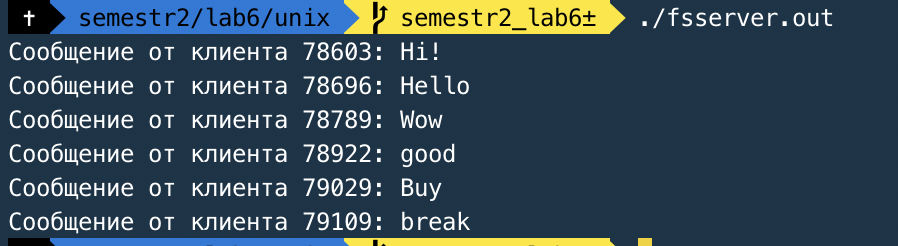
\includegraphics{server1}

\newpage

Запускаем приложения клиентов, отправляем сообщения, при отправке сообщения break сервер заканчивает работу:

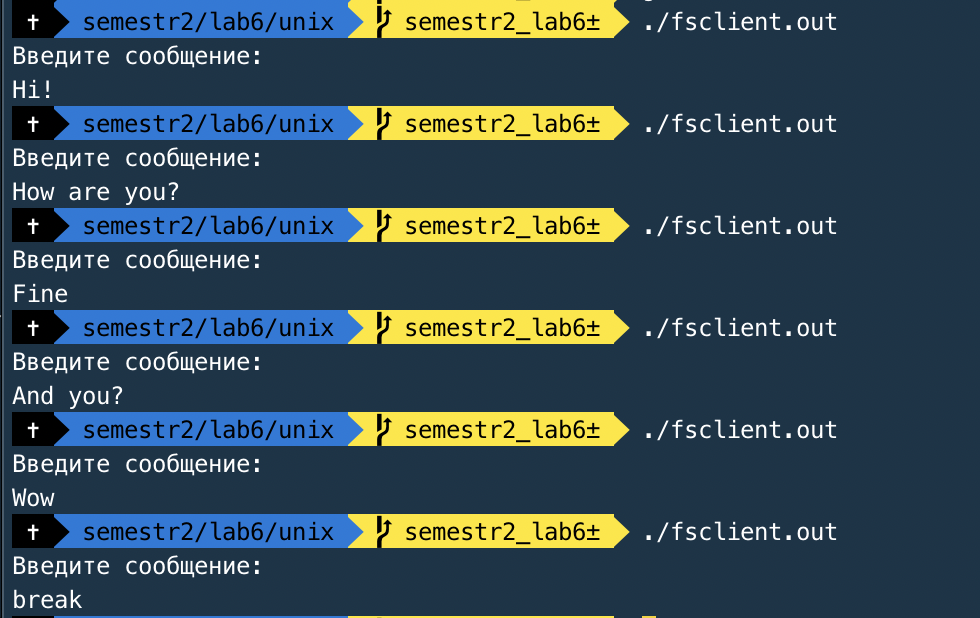
\includegraphics{client1}

\newpage

\textbf{Задание 2:} Написать приложение по модели клиент-сервер, осуществляющее взаимодействие параллельных процессов, которые выполняются на разных компьютерах. Для взаимодействия с клиентами сервер должен использовать мультиплексирование. Сервер должен обслуживать запросы параллельно запущенных клиентов. При демонстрации работы программного комплекса необходимо запустить несколько клиентов (не меньше 5) и продемонстрировать, что сервер обрабатывает обращения каждого запущенного клиента.

\begin{lstlisting}[caption=Код сервера]
#include <stdio.h>
#include <stdlib.h>
#include <errno.h>
#include <strings.h>
#include <sys/types.h>
#include <sys/socket.h>
#include <netinet/in.h>
#include <unistd.h>

#define MSG_SIZE 256
#define LISTENQ 1024

int maxi, maxfd;

// Соединение с новым клиентом
int newClient(int listensock, int client[FD_SETSIZE], int id[FD_SETSIZE], fd_set *allset, fd_set *reset)
{
  // Индекс
  int i;
  int connfd;
  char pid[MSG_SIZE];

  if (FD_ISSET(listensock, reset))
  {
    // Установка соединения в ответ на запрос клиента
    // Так как нас не интересуют данные об адресе клиента
    // передаем значения NULL в предпоследнем и последнем параметрах
    int connfd = accept(listensock, NULL, NULL);
    if (connfd < 0)
    {
      printf("%s", strerror(errno));
      return errno;
    }
    // Функция accept() возвращает новый сокет, открытый
    // для обмена данными с клиентом, запросившим соединение

    // Сохраняем дескриптор в первый свободный
    for (i = 0; i < FD_SETSIZE; i++)
    {
      if (client[i] < 0)
      {
        client[i] = connfd;
        break;
      }
    }

    if (i == FD_SETSIZE)
    {
      printf("Достигнуто максимальное число клиентов");
      return errno;
    }

    // Добавление нового дескриптора
    FD_SET(connfd, allset);

    // Максимальный для функции select
    if (connfd > maxfd)
      maxfd = connfd;

    // Максимальный индекс в массиве клиентов
    if (i > maxi)
      maxi = i;

    read(connfd, pid, MSG_SIZE);
    id[i] = atoi(pid);
    printf("Клиент %d подключился\n", id[i]);
  }
  return errno;
}

int readMsg(int client[FD_SETSIZE], int id[FD_SETSIZE], fd_set *allset, 
							fd_set *reset)
{
  int n, i;
  int sockfd;
  char msg[MSG_SIZE];
  // Проверяем все клиенты на наличие данных, пока не дошли до конца
  // или не закончились дескрипторы готовые для чтения
  for (i = 0; i <= maxi; i++)
  {
    // Если не пустой
    if ((sockfd = client[i]) > 0)
    {
      // Установлен ли бит?
      if (FD_ISSET(sockfd, reset))
      {
        // Соединение закрыто клиентом
        if ((n = read(sockfd, msg, MSG_SIZE)) == 0)
        {
          // Закрываем сокет
          close(sockfd);
          // Сброс бита
          FD_CLR(sockfd, allset);
          // Освобождаем ячейку в массиве клиентов
          client[i] = -1;
          printf("Клиент %d отключился\n", id[i]);
        }
        else
        {
          // Сообщение клиенту о доставке сообщения
          write(sockfd, "OK", 2);
          // Установка символа конца строки и вывод сообщения на экран
          msg[n] = 0;
          printf("Сообщение от клиента %d: %s", id[i], msg);
        }
      }
    }
  }
  return errno;
}

int main(int argc, char ** argv)
{
  int listensock;
  int client[FD_SETSIZE];
  int id[FD_SETSIZE];
  fd_set reset, allset;
  // Структура предназначен для хранения адресов в формате Интернета
  struct sockaddr_in server;

  if (argc < 2)
  {
    fprintf(stderr, "Использование: %s <port_number>\n", argv[0]);
    return 1;
  }

  // Создание сетевого сокета (домен AF_INET)
  // Тип сокета -- SOCK_STREAM, сокет должен быть потоковым
  // Протокол -- 0, протокол выбирается по умолчанию
  listensock = socket(AF_INET, SOCK_STREAM, 0);
  if (listensock < 0)
  {
    printf("%s", strerror(errno));
    return errno;
  }

  // Укажем семейство адресов, которыми мы будем пользоваться
  server.sin_family = AF_INET;
  // Укажем адрес (наша программа-сервер зарегистрируется на всех адресах
  // машины, на которой она выполняется)
  server.sin_addr.s_addr = INADDR_ANY;
  // Укажем значение порта. Функция htons() переписывает 
  // двухбайтовое значение порта так, чтобы порядок байтов 
  // соответствовал принятому в Интернете
  server.sin_port = htons(atoi(argv[1]));

  // Связывание сокета с заданным адресом
  // bind(дескриптор сокета, указатель на структуру, длина структуры)
  if (bind(listensock, (struct sockaddr *) &server, sizeof(server)) < 0)
  {
    printf("%s", strerror(errno));
    return errno;
  }

  // Переводим сервер в режим ожидания запроса на соединение
  // Второй параметр - максимальное число 
  // обрабатываемых одновременно соединений
  listen(listensock, LISTENQ);

  // Инициализация значения
  maxfd = listensock;
  // Индекс в массиве клиентов (наибольший используемый)
  maxi = -1;
  // Массив дескрипторов присоединенного сокета для каждого клиента
  for (int i = 0; i < FD_SETSIZE; i++)
    client[i] = -1; // -1 означает, что элемент свободен

  // Сбрасываем все биты в allset
  FD_ZERO(&allset);
  // Устанавливаем бит для listensock в allset
  FD_SET(listensock, &allset);

  while(1)
  {
    // Присваивание значения структуре
    reset = allset;
    // select() ждет пока не будет установлено новое клиентское 
    // соединение или на существующем не прибудут данные
    // select(количество проверяемых дескрипторов, 2-4 наборы 
    // дескрипторов, которые следует проверять, интервал времени, 
    // по прошествии которого она вернет управление в любом случае)
    select(maxfd + 1, &reset, NULL, NULL, NULL);

    if (newClient(listensock, client, id, &allset, &reset) ||
		  readMsg(client, id, &allset, &reset))
      return errno;
  }

  // Закрываем сокет
  close(listensock);

  return errno;
}
\end{lstlisting}

\begin{lstlisting}[caption=Код клиента]
#include <stdio.h>
#include <stdlib.h>
#include <errno.h>
#include <strings.h>
#include <sys/types.h>
#include <sys/socket.h>
#include <netinet/in.h>
#include <netdb.h>
#include <unistd.h>

#define MSG_SIZE 256

int main(int argc, char ** argv)
{
  struct sockaddr_in server;
  struct hostent *host;
  char msg_client[MSG_SIZE], msg_server[MSG_SIZE];
  char id[10];
  sprintf(id, "%d", getpid());
  id[strlen(id)] = 0;

  if (argc < 3)
  {
     fprintf(stderr, "Использование: %s <hostname> <port_number>\n", 
     								argv[0]);
     return 1;
  }

  // Создание сетевого сокета (домен AF_INET)
  // Тип сокета -- SOCK_STREAM, сокет должен быть потоковым
  // Протокол -- 0, протокол выбирается по умолчанию
  int sock = socket(AF_INET, SOCK_STREAM, 0);
  if (sock < 0)
  {
    printf("%s", strerror(errno));
    return errno;
  }

  // Преобразование доменного имени сервера в его сетевой адрес
  host = gethostbyname(argv[1]);
  if (host == NULL)
  {
    printf("%s", strerror(errno));
    return errno;
  }

  // Укажем семейство адресов, которыми мы будем пользоваться
  server.sin_family = AF_INET;
  // Укажем адрес (наша программа-сервер зарегистрируется на всех адресах
  // машины, на которой она выполняется)
  memcpy(&server.sin_addr, host->h_addr_list[0], host->h_length);
  // Укажем значение порта. Функция htons() переписывает 
  // двухбайтовое значение порта так, чтобы порядок байтов 
  // соответствовал принятому в Интернете
  server.sin_port = htons(atoi(argv[2]));

  // Установка соединения
  if (connect(sock, (struct sockaddr *) &server, sizeof(server)) < 0)
  {
    printf("%s", strerror(errno));
    return errno;
  }
  write(sock, id, strlen(id));

  // Пока не сообщение "break"
  while (strcmp(msg_client, "break\n"))
  {
    memset(msg_client, 0, MSG_SIZE);
    printf("Введите сообщение:\n");
    fgets(msg_client, MSG_SIZE, stdin);
    // Для записи данных - write
    write(sock, msg_client, strlen(msg_client));

    // Заполнение массива нулями
    memset(msg_server, 0, MSG_SIZE);
    // Для чтения данных из сокета - read
    read(sock, msg_server, MSG_SIZE);
    printf("%s\n", msg_server);
  }
  // Закрываем сокет
  close(sock);

  return 0;
}
\end{lstlisting}

\newpage

Запускаем приложение сервера и принимаем сообщения от клиентов:

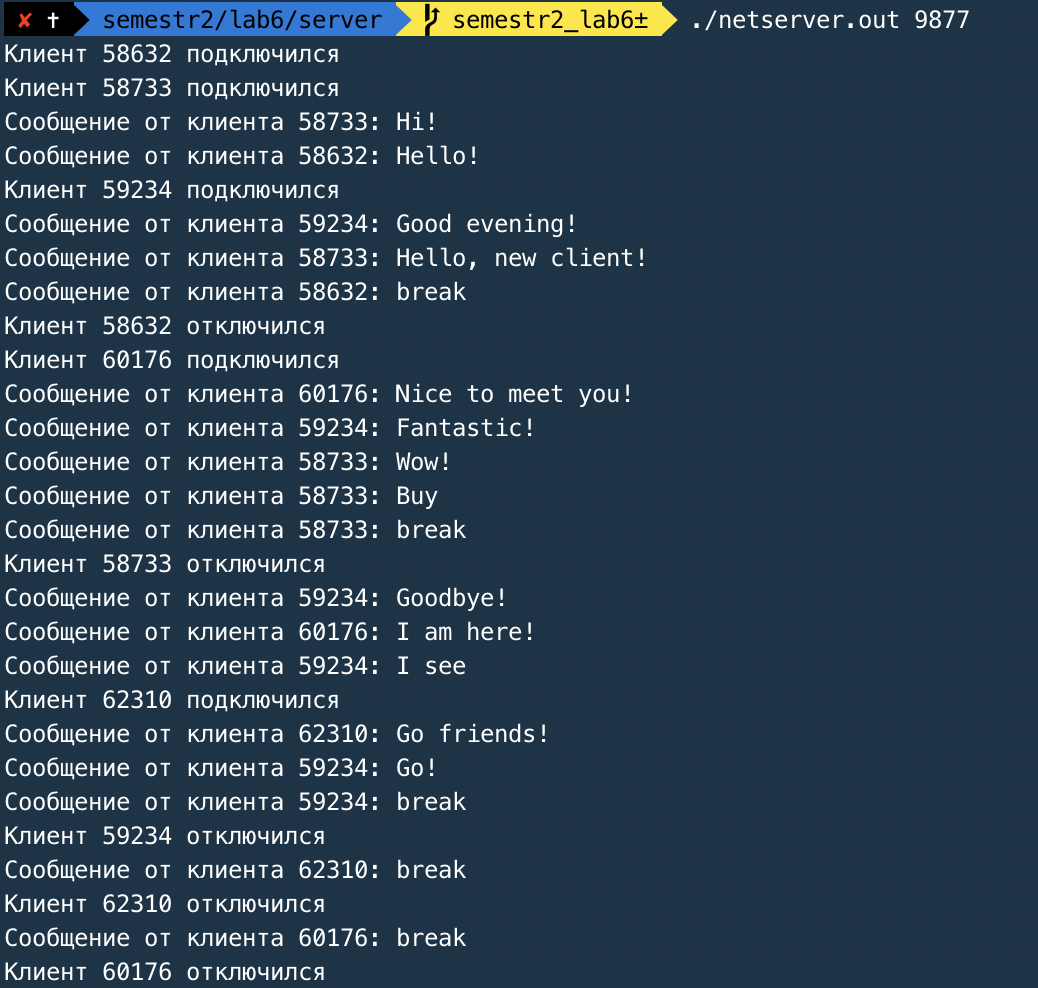
\includegraphics[scale=0.9]{server21}

\newpage

Запускаем приложения клиентов, при каждом новом подключении сервер выводит сообщение об этом. Далее несколько клиентов отправляют сообщения, могут завершиться, затем вновь возобновить работу. 

При этом новому клиенту присваивается первый свободный номер. 

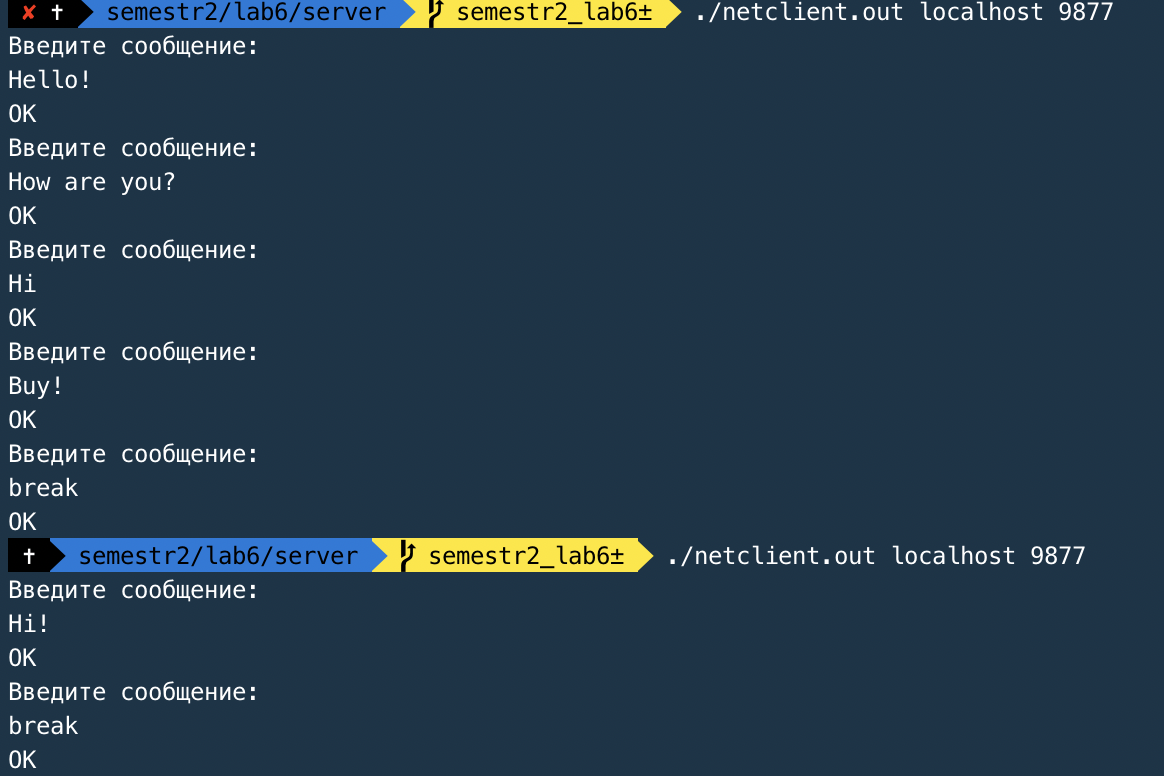
\includegraphics[scale=0.8]{client21}

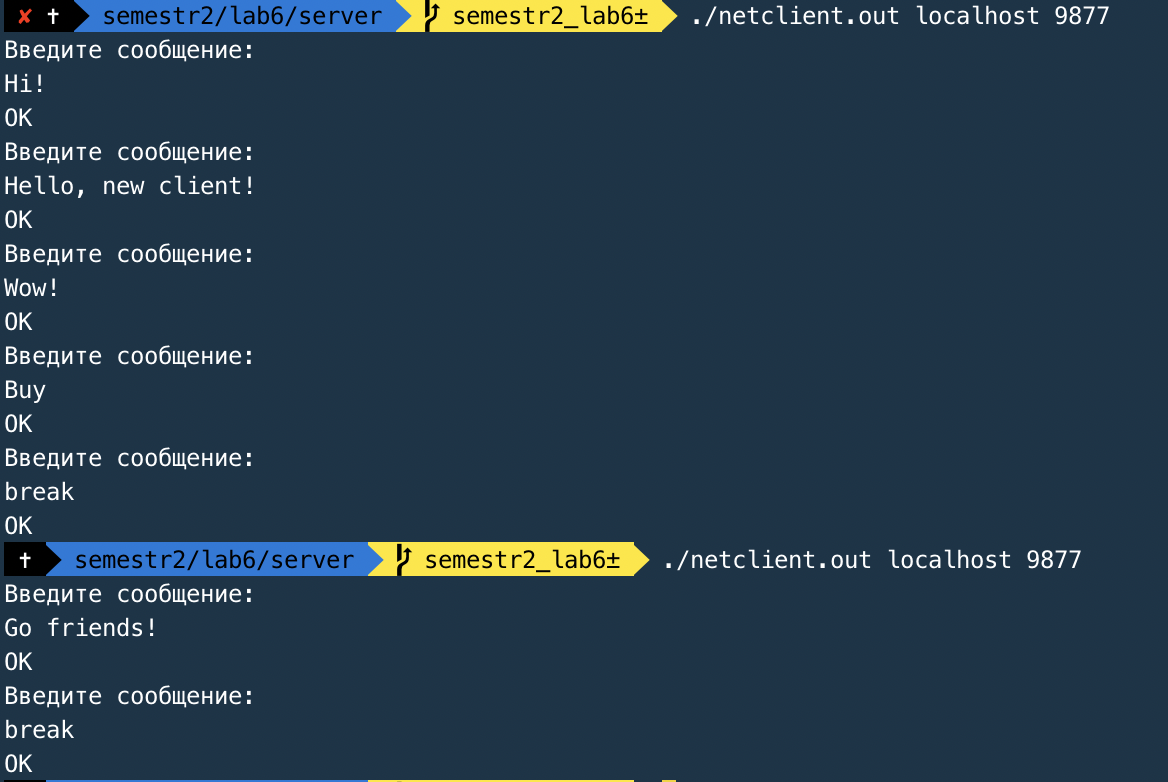
\includegraphics[scale=0.8]{client22}

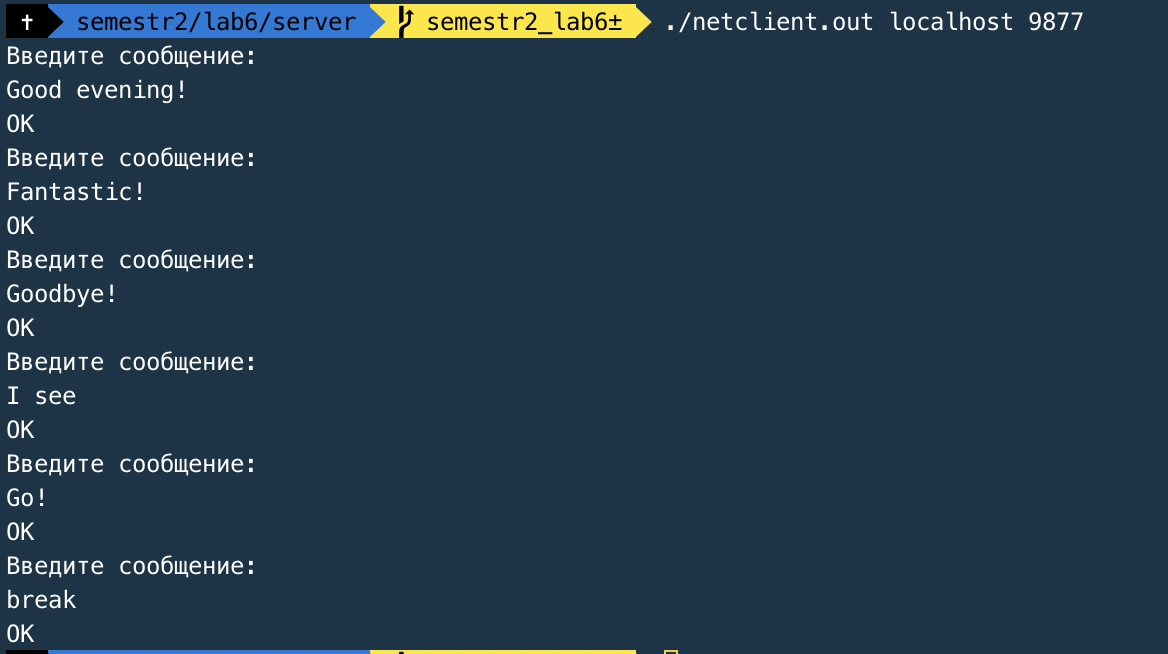
\includegraphics[scale=0.8]{client23}

Максимально одновременно можно запустить FD$\_$SETSIZE = 256 клиентов. Запустим 5 клиентов одновременно проверим работу. 

Сервер:

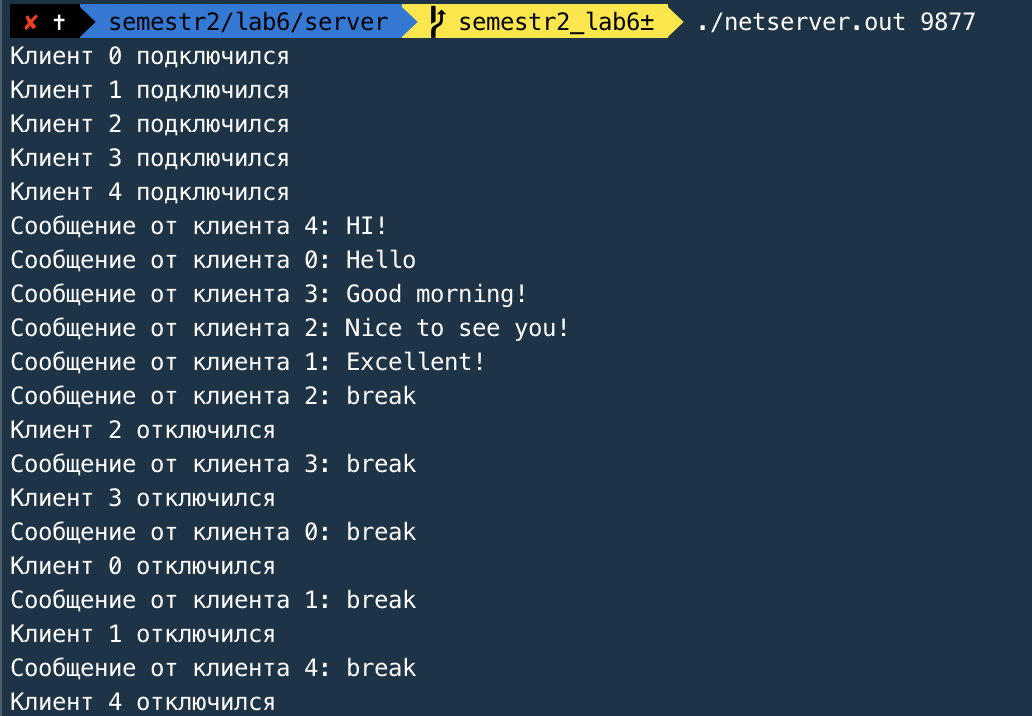
\includegraphics[scale=0.8]{server22}

\newpage

Клиенты:

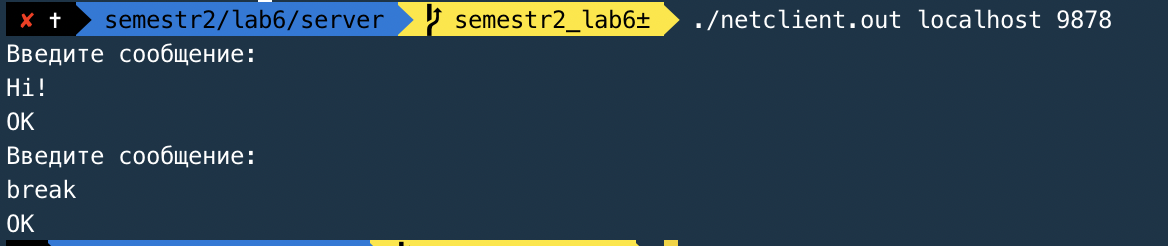
\includegraphics[scale=0.8]{client24}

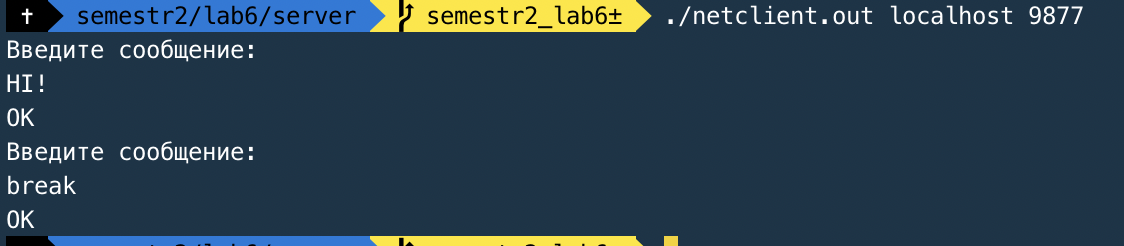
\includegraphics[scale=0.8]{client25}

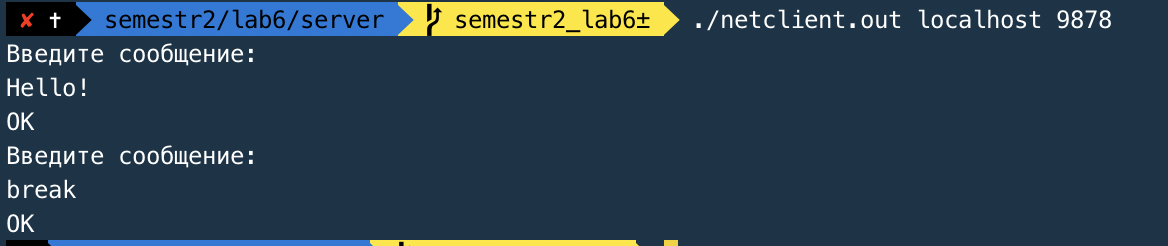
\includegraphics[scale=0.8]{client26}

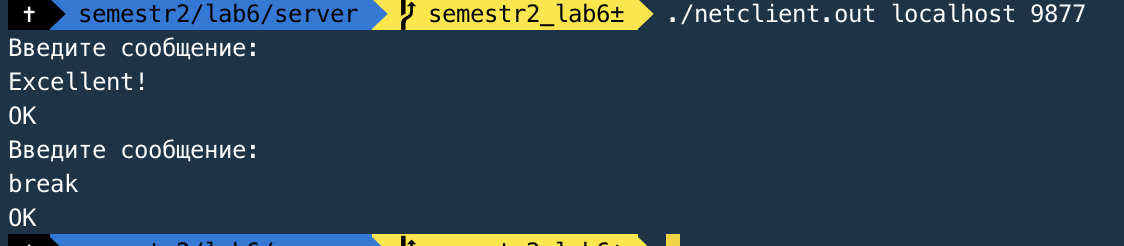
\includegraphics[scale=0.8]{client27}

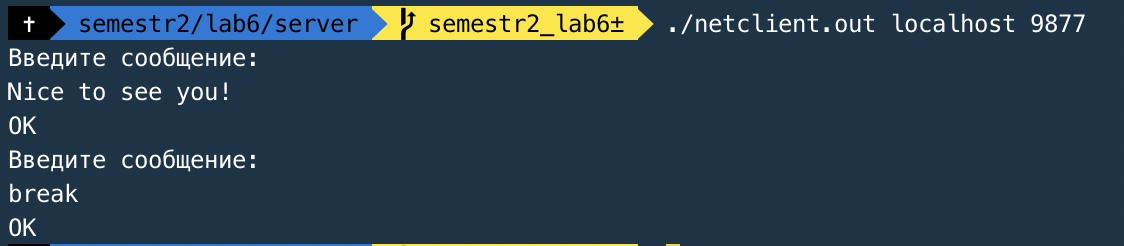
\includegraphics[scale=0.8]{client28}

\end{document}